
\chapter{Heating-Cooling Asymmetry: Discrete Case}\label{cap:results-discrete}

Experiments showed that heating is faster than cooling in Langevin systems \cite{ibanez-2024} and theoretical studies showed that this asymmetry also exist in quantum systems \cite{tejero-2025}. However, understanding how quantum resources affect heating-cooling asymmetry is still an open question. In this chapter, we will investigate quantum coherence and entanglement effects on the asymmetry. For that, we consider two interacting qubits coupled to a global bosonic bath. However, before we discuss the results of this work, it is important to present the quantum correlations we will investigate, which is done in Sec. \ref{sec:correlations}. Then, in Sec. \ref{sec:qubits}, we examine characteristics of the two interacting qubits model and discuss its thermalization process. After this introductions, we will be able to analyse our results in Sec. \ref{sec:asymmetry-qubit}.


\section{Quantum Coherence and Entanglement} \label{sec:correlations}
% correlations for this work: coherence + entanglement
% how to measure them?
% how they affect ergotropy and entropy?

One of the basic properties of quantum systems is the possibility of being in a superposition state, for example $\ket{\psi} = a \ket{0} + b \ket{1}$, where $\ket{0} = (1,0)^T$ and $\ket{1} = (0,1)^T$ form the computational basis. In the density matrix form, this state becomes
\begin{equation}
    \rho = 
    \begin{bmatrix}
        |a|^2 & ab^*\\
        a^* b & |b|^2
    \end{bmatrix},
\end{equation}

\noindent where the off-diagonal elements represent the coherences of the state. In other words, we call coherent states the ones with off-diagonal elements in their density matrices while the incoherent states are represented by diagonal density matrices \cite{streltsov-2017, baumgratz-2014}. However, coherence is a basis dependent quantity, which implies that we must fix one basis to define it. Usually this reference basis is selected according to the physical problem, for example, the energy eigenbasis is the most used in studies of thermodynamic processes. It is important to emphasize that the off-diagonal elements cannot assume arbitrary values, because the positive semi-definite condition of the density matrix must be preserved, which implies that
\begin{equation}
    |{\rho}_{ij}|^2 \leq {\rho}_{ii} {\rho}_{jj},
    \label{eq:coherence-positivity}
\end{equation}

\noindent where the subindexes identifies the density matrix element. 

There are different ways to measure the coherence of a state, being the relative entropy of coherence one of them. It is defined as \begin{equation}
    \begin{split}
        C_R ({\rho}) &= \min_{{\sigma} \in I} D[{\rho} || {\sigma}] = S({\rho}_d) - S({\rho}),
    \end{split}
    \label{eq:relative-coherence}
\end{equation}

\noindent that is a minimization over all the set of incoherent states $I$ of the relative entropy between the state we want to measure ${\rho}$ and the incoherent state ${\sigma}$ \cite{streltsov-2017}. The last equality is obtained by using that we can separate any density matrix into a diagonal part ${\rho}_d = \sum_i \ket{i}\bra{i} {\rho} \ket{i}\bra{i}$ and a coherent part, which allow us to rewrite the relative entropy as $D[{\rho} || {\sigma}] = S({\rho}_d) - S({\rho}) + D[{\rho}_d || {\sigma}]$. The minimization over ${\sigma}$ of this expression, means that ${\rho}_d = {\sigma}$, resulting the last equality in Eq. \eqref{eq:relative-coherence}. Using this measure, we can prove that the maximally coherent state have maximum values of the off-diagonal elements, resulting in the pure state $\ket{\psi_{MCS}} = d^{-1} \sum_{i=0}^{d} \ket{i}$ that has $C_R ({\rho}) = \log d$ \cite{baumgratz-2014}.

Coherence have non-trivial consequences in thermodynamic processes and, for this reason, investigating its effects in the heating-cooling asymmetry can be interesting. One example of how coherence affects thermodynamics, is that coherence in the energy basis can increase the ergotropy of the state, which means it can be exploited as a resource for work extraction \cite{francica-2020}. However, there are cases where coherence can be detrimental for physical processes, such as in some stages of quantum batteries operations \cite{campaioli-2024} and in thermal relaxation processes \cite{krissia-2024}.

When we have two of more quantum systems, they can share information through classical and quantum correlations. There are a variety of quantum correlations that can be organised as a hierarchy \cite{adesso-2016}, being coherence the necessary condition for all of them. In this work, we will only study the bipartite entanglement (that is the entanglement between two parts). Consider a composite system whose global state can be separated into two subsystems, such as $\ket{\psi}_{AB} = \ket{\alpha}_A \otimes \ket{\beta}_B$, meaning the subsystems are not entangled. On the other hand, when we cannot obtain the global state by any combination of local states $\ket{\alpha}_A$ and $\ket{\beta}_B$, the global state $\ket{\psi}_{AB}$ is said to be entangled \cite{adesso-2016}. In the density matrices formulation, separable states can be decomposed into local pure mixed states,
\begin{equation}
    {\rho} = \sum_i p_i {\rho}_i^A \otimes {\rho}_i^B.
    \label{eq:rho-separavel}
\end{equation}

\noindent As a consequence, the state is entangled if the decomposition in Eq. \eqref{eq:rho-separavel} is not possible \cite{adesso-2016}.

A usual measure of correlations is the mutual information defined as
\begin{equation}
    \mathcal{M}(\rho_{AB}) = S({\rho}_A) + S({\rho}_B) - S({\rho}_{AB}),
    \label{eq:mutual-info}
\end{equation}

\noindent where $S(\rho)$ is the von Neumann entropy, ${\rho}_A$ and ${\rho}_B$ are parts of the global state ${\rho}_{AB}$ \cite{chuang-book}. However, this quantity indicates how much information is shared through both classical and quantum correlations, meaning it cannot be used alone as a signature of quantumness. Because, in this work, we will only use bipartite entanglement, we can use a more specific quantifier. The entanglement of formation (EoF), that is defined as
\begin{equation}
    E_f ({\rho}) = H \left( \frac{1+\sqrt{1-C({\rho})^2}}{2} \right),
    \label{eq:eof}
\end{equation}

\noindent where $H(x) = -x\log_2(x) - (1-x)\log_2 (1-x)$ is the Shannon entropy and
\begin{equation}
    C({\rho}) = \max\{ 0, \lambda_1 - \lambda_2 - \lambda_3 - \lambda_4 \},
    \label{eq:concurrence}
\end{equation}

\noindent is the concurrence for the case of two qubits\footnote{The general definition can be found in Ref. \cite{adesso-2016}}, where $\lambda_i > \lambda_j$ for $i<j$ are the square root of the eigenvalues of the matrix $R = \rho \tilde{\rho}$. To find $R$, first we take complex conjugation of each matrix element obtaining $\rho^*$ and then we compute the time-reversed matrix $\tilde{\rho} = (\sigma_y \otimes \sigma_y) \rho^* (\sigma_y \otimes \sigma_y)$ \cite{rigolin-2010}.

Entanglement is widely used as quantum resource in communication and computation \cite{chitambar-2019}, and it can also bring advantages in thermodynamics processes. For example, refrigerators can make entangled systems reach lower temperatures than no-correlated states \cite{alba-2026}. Another example, is that entanglement can help extract more work in quantum batteries \cite{alicki-2013}.

There are other methods to quantify entanglement and coherence in quantum systems, but the presented discussion is enough for this work. In the next section, we will explain the thermal relaxation of the two interacting qubits model and will present our results in Sec. \ref{sec:asymmetry-qubit}.


%%%%%%%%%%%%%%%%%%%%%%%%%%%%%%%%%%%%%%%%%%%%%%%%%%%%%%%%%%%%%%%%%%%%%%%%%

\section{Thermal Relaxation of Two Interacting Qubits}\label{sec:qubits}

The two interaction qubits model we will use can be described by
\begin{equation}
    H_S = - \frac{\omega_0}{2} \sigma_{1}^{z} -  \frac{\omega_0}{2} \sigma_{2}^{z} + J [\sigma_{1}^{+} \sigma_{2}^{-} + \sigma_{1}^{-} \sigma_{2}^{+}],
    \label{eq:HS-qubit}
\end{equation}

\noindent where $\sigma_{i}^{+} = \ket{1}\bra{0}$, $\sigma_{i}^{-} = \ket{0}\bra{1}$, and $\sigma_{i}^{z}$ is the Pauli matrix in z acting on qubit $i$. We will consider that both qubits have the same energy gap $\frac{\omega_0}{2}$. The qubits can exchange energy and information through the XX-interaction model with strength $J$ \cite{medina-2024, rigolin-2010}. Depending on the value of $J$, the final state of the dynamics can have more coherence and even stronger correlations, such as entanglement, which will be discussed later in this section.

\begin{figure}[t!]
    \centering
    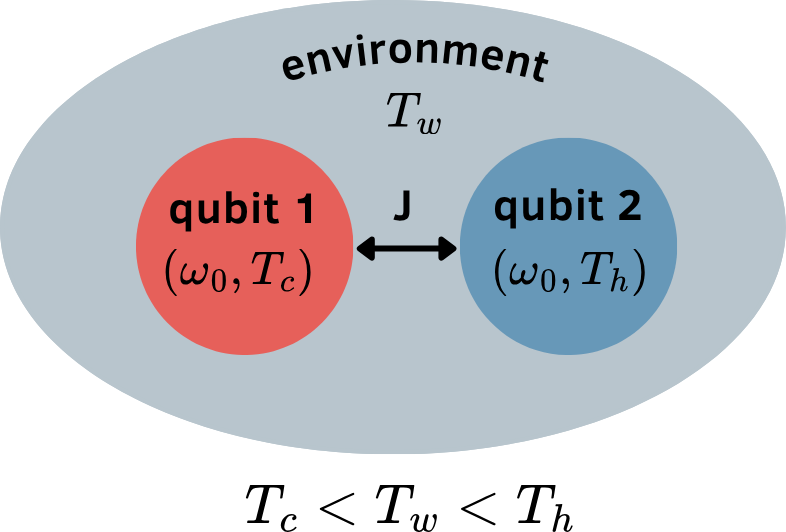
\includegraphics[width=0.35\linewidth]{Images/Qubits/model-2-qubits.png}
    \caption{Illustration of two interacting qubits in contact wit a global bath. The red qubit is at a colder temperature $T_c$ and will heat up to the bath's temperature $T_w$. The blue qubit is at a hotter temperature $T_h$ and will cool down to the bath's temperature $T_w$. The qubits can interact with a strength $J$.}
    \label{fig:model-2-qubits}
\end{figure}

To study the heating-cooling asymmetry with this model, we will consider that one qubit is initially at a colder temperature $T_c$ and the other qubit is initially at a hotter temperature $T_h$. Because the bath is at an intermediate temperature $T_w$, the colder qubit will heat up and the hotter qubit will cool down. To genuinely study heating and cooling, it is important to assure each qubit is at a thermal state so we can define a physical temperature to it. If we add off-diagonal elements in each qubit's density matrix, that is, coherence, they would not be thermal states and the terms ``heating” and ``cooling” become inaccurate. Therefore, to study the effects of coherence in heating-cooling asymmetry with this model, we will use an initial X-state
\begin{equation}
    \rho = \rho_{c} \otimes \rho_{h} + \chi,
\end{equation}

\noindent where $\rho_c$ and $\rho_h$ are the thermal states of the cold and hot qubits, respectively, and $\chi$ is a matrix defined in computational basis as
\begin{equation}
    \chi = e \ket{01}\bra{10} + e^* \ket{10}\bra{01} + f \ket{00}\bra{11} + f^* \ket{11}\bra{00},
\end{equation}

\noindent which means it contains the coherences of the global state. These coherences only exist for the global state because $\text{Tr}_c[\chi] = \text{Tr}_h[\chi] = 0$. This particular format is important because it allow us to include coherences while keeping thermal local states for each qubit, which means that $\text{Tr}_c[\rho] = \rho_h$ and $\text{Tr}_h[\rho] = \rho_c$.

As discussed in Sec. \ref{sec:correlations}, the positivity of every density matrix imposes the constraint shown in Eq. \eqref{eq:coherence-positivity} on the off-diagonal elements. In our case, the matrix form of the initial density matrix of our state is
\begin{equation}
    \rho = 
    \begin{bmatrix}
        \frac{e^{\omega_0 (\beta_c + \beta_h)/2}}{\mathcal{Z}_c \mathcal{Z}_h} & 0 & 0 & f\\
        0 & \frac{e^{\omega_0 (\beta_c - \beta_h)/2}}{\mathcal{Z}_c \mathcal{Z}_h} & e & 0\\
        0 & e^* & \frac{e^{-\omega_0 (\beta_c - \beta_h)/2}}{\mathcal{Z}_c \mathcal{Z}_h} & 0\\
        f^* & 0 & 0 & \frac{e^{-\omega_0 (\beta_c + \beta_h)/2}}{\mathcal{Z}_c \mathcal{Z}_h}
    \end{bmatrix},
    \label{eq:initial-rho}
\end{equation}

\noindent where $\beta_i = 1/T_i$ and the partition function is $\mathcal{Z}_i = 2 \cosh(\beta_i \omega_0 / 2)$ with $i = (c,h)$. After its diagonalization, we obtain that the maximum value for $|e|$ and $|f|$ is $1/\mathcal{Z}_c \mathcal{Z}_h$. Even though this initial state can have coherence, this limitation for the off-diagonal elements makes impossible to have entanglement according to the requirements in Ref. \cite{ali-2010}.

To study the thermal relaxation of this model and initial state, we will use the Davies maps presented in Sec. \ref{sec:davies-maps}. As we previously discussed, the steady state of this dynamics is always a thermal state, which enable us to find that
\begin{equation}
    \begin{split}
        \rho_{ss}^{G} &= \frac{e^{-\beta_w H_S}}{\mathcal{Z}_S}\\
        &= \frac{1}{\mathcal{Z}_S}
        \begin{bmatrix}
            e^{\beta_w \omega_0} & 0 & 0 & 0\\
            0 & e^{\beta_w J} & 0 & 0\\
            0 & 0 & e^{-\beta_w J} & 0\\
            0 & 0 & 0 & e^{-\beta_w \omega_0}
        \end{bmatrix}\\
        &= \frac{1}{\mathcal{Z}_S}
        \begin{bmatrix}
            e^{\beta_w \omega_0} & 0 & 0 & 0\\
            0 & \cosh(\beta_w \omega_0) & -\sinh(\beta_w J) & 0\\
            0 & -\sinh(\beta_w J) & \cosh(\beta_w \omega_0) & 0\\
            0 & 0 & 0 & e^{-\beta_w \omega_0}
        \end{bmatrix},
    \end{split}
    \label{eq:global-steady-state}
\end{equation}

\begin{figure}[b!]
    \centering
    
\includegraphics[width=\linewidth]{Images/Qubits/correlations-J.png}
    \caption{Quantifiers of correlations in the global thermal state (Eq. \eqref{eq:global-steady-state}) caused by the qubits interaction. Concurrence (left), entanglement of formation (right), and mutual information as a function of the interaction parameter $J$.}
    \label{fig:C-EoF-MI}
\end{figure}

\noindent where $\mathcal{Z}_S = 2(\cosh(\beta_w \omega_0) + \cosh(\beta_w J))$ is the partition function with $\beta_w = 1/T_w$ and $H_S$ being the Hamiltonian from Eq. \eqref{eq:HS-qubit}. The second equality is in the energy basis and the last equality is in the computational basis. Now that we know the global steady state, we go back to the discussion about the emergence of entanglement due to the interaction of the qubits. We can use entanglement of formation (defined in Eq. \eqref{eq:eof}) to identify which parameter we can obtain entanglement between the qubits. First, we need to compute the concurrence (defined in Eq. \eqref{eq:concurrence}) for this state. In Appx. \ref{apx:concurrence}, we find that the square root of the eigenvalues of $R$ (defined in Sec. \ref{sec:correlations}) are in decreasing order $\lambda_1 = e^{\beta_w J}/\mathcal{Z}_S$, $\lambda_2 = \lambda_3 = 1/\mathcal{Z}_S$, and $\lambda_4 = e^{-\beta_w J}/\mathcal{Z}_S$. Fig. \ref{fig:C-EoF-MI} show that concurrence increase for $J>0.8814$, resulting in an increase of the entanglement of formation. So we conclude that this model can have entanglement for stronger interaction between the qubits. Additionally, it is also possible to compute the mutual information defined in Eq. \eqref{eq:mutual-info} and shown the right plot of Fig. \ref{fig:C-EoF-MI}. We see that the mutual information increase for higher $J$, but it is bigger than zero before entanglement of formation, which means that other types of correlations emerge even for weak interaction between the qubits.

\begin{figure}[t]
    \centering
    
\includegraphics[width=0.5\linewidth]{Images/Qubits/qubit-final-T.png}
    \caption{Final temperature of the qubits (Eq. \eqref{eq:qubit-final-T}) as a function of the interaction parameter $J$.}
    \label{fig:qubit-final-T}
\end{figure}

However, the appearance of correlation between the qubits affects their final states. When we trace out one of the qubits from the global steady state (Eq. \eqref{eq:global-steady-state}), we find the local steady state 
\begin{equation}
    \rho_{ss}^q = \frac{1}{\mathcal{Z}_q}
    \begin{bmatrix}
        e^{\beta_w \omega_0} + \cosh (\beta_w J) & 0\\
        0 & e^{-\beta_w \omega_0} + \cosh (\beta_w J)
    \end{bmatrix},
\end{equation}

\noindent where $\mathcal{Z}_q = 2 \cosh(\beta_f \omega_0) + 2 \cosh(\beta_f J)$. Because in a global bath both qubits equilibrate to the same local temperature, it makes no difference which one we trace out. From the final state of the qubit, we can compute its final temperature, obtaining
\begin{equation}
    \beta_{f}^{q} = \frac{1}{\omega_0} \ln \left( \frac{e^{\beta_w \omega_0} + \cosh (\beta_w J)}{e^{-\beta_w \omega_0} + \cosh (\beta_w J)} \right),
    \label{eq:qubit-final-T}
\end{equation}

\noindent which is smaller than the bath's temperature for $J>0$, as shown in Fig. \ref{fig:qubit-final-T}. It must be emphasised that the global system thermalises to the bath's temperature, as we calculated in Eq. \eqref{eq:global-steady-state}. However, because the interaction between the qubits generates correlations (as signalised by the mutual information), tracing out one of them erases part of the information, which changes the qubit's populations resulting in a different final temperature.


Now that we discussed the interaction model between the qubits and the structure of the initial and final states, we can analyse how the heating-cooling asymmetry behaves for our system. In the next section, we present our results and how we obtained them. 




%%%%%%%%%%%%%%%%%%%%%%%%%%%%%%%%%%%%%%%%%%%%%%%%%%%
\section{Asymmetry for Two Interacting Qubits}\label{sec:asymmetry-qubit}

Before solving the dynamics for our model and analyse the asymmetry, it is important to guarantee we are making a fair comparison between heating and cooling. In this sense, we must choose initial states for the qubits that are thermodynamically equivalent, which is not the same as having equidistant initial temperatures from equilibrium temperature. Given that the asymmetry only appears for far-from-equilibrium systems, the criteria we will use for thermodynamic equivalence will be the nonequilibrium free energy defined by Eq. \eqref{eq:fneq}. As we discussed in Sec. \ref{sec:thermo-variables}, states with the same nonequilibrium free energy also have the same relative entropy from equilibrium. So, we choose a colder ($\rho_c$) and hotter ($\rho_c$) initial states for the qubits that have the same relative entropy from their final local steady state ($\rho_{ss}^q$),
\begin{equation}
    D[\rho_c || \rho_{ss}^{q}] = D[\rho_h || \rho_{ss}^{q}] = D_0,
    \label{eq:same-D-qubit}
\end{equation}

\begin{figure}[b!]
    \centering
    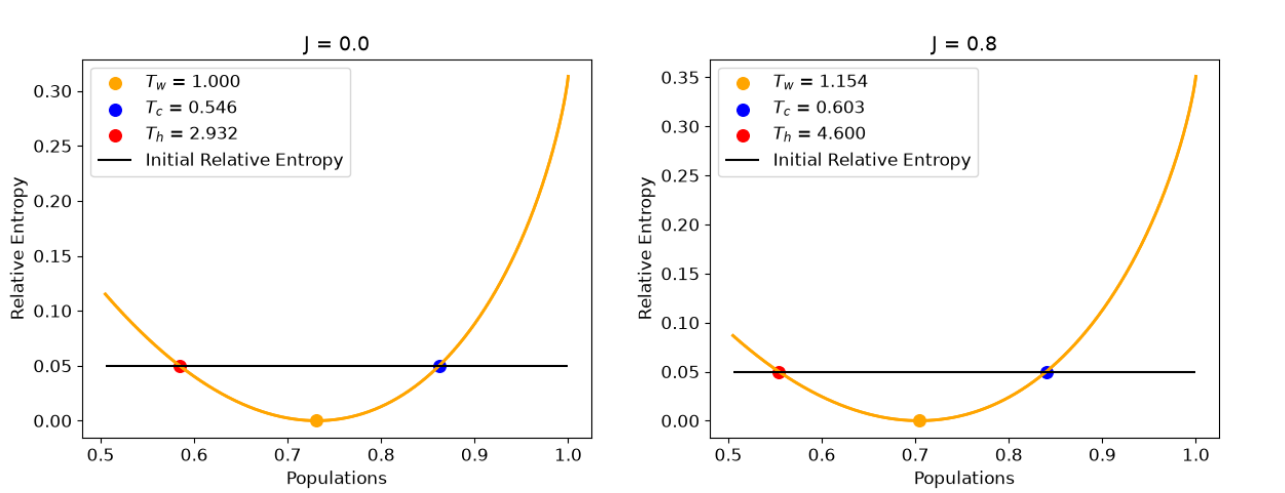
\includegraphics[width=\linewidth]{Images/Qubits/same-D-qubits.png}
    \caption{Relative entropy of a thermal qubit and its equilibrium state as a function of its ground state population. The orange curve is obtained by varying the qubit's temperature and the orange dot corresponds to the equilibrium state. The black line indicates the chosen initial relative entropy that both hot (red dot) and cold (blue dot) qubits must have. The left plot is the no-interaction case, while the right plot show the interaction case with $J = 0.8$.}
    \label{fig:same-D-qubits}
\end{figure}

\noindent where we use the relative entropy definition from Eq. \eqref{eq:relative-entropy}. This equality can be numerically solved by varying the initial temperature of the qubit's thermal state and computing its relative entropy from $\rho_{ss}^q$. This will result is the orange curve in Fig. \ref{fig:same-D-qubits}, where the orange dot indicates the equilibrium state with inverse temperature $\beta_{f}^{q}$. Then, we can find the points where this orange curve is equal to the initial relative entropy $D_0$ (black line). Using that the population of the ground state ($\bra{0}\rho\ket{0} = \exp(\omega_0/2T_i)/2\cosh(\omega_0/2T_i)$ with $i=(c,h)$), we can find the initial cold (blue dot) and hot (red dot) temperatures that the qubits must have to be thermodynamically equivalent.


With this initialization of our system, we can analyse the heating and cooling asymmetry. In the next figures, heating and cooling are represented in red and blue, respectively. Dashed lines indicate the non-interaction case ($J = 0$), while solid lines represent the interaction case without entanglement ($J = 0.8$). The degree of completion (defined by Eq. \eqref{eq:completion}) is shown in Fig. \ref{fig:completion-xx} for the case without initial coherence (left) and the case with maximum initial coherence (right). When comparing heating and cooling, the red lines are above their corresponding blue lines, so we conclude that heating is faster than cooling. Using this same idea, we see that the interaction between qubits allows a faster relaxation. Furthermore, only for the interaction case, the initial coherence seems to affect the intermediary dynamics by delaying cooling, which increases the asymmetry while keeping the total relaxation time unchanged. These same observations can be also obtained from the statistical velocity (defined by Eq. \eqref{eq:velocidade}) shown in Fig. \ref{fig:velocity-xx}. In addition to this, note that the interaction case have many oscillations in both degree of completion and statistical velocity, which will be discussed later.

\begin{figure}[t]
    \centering
    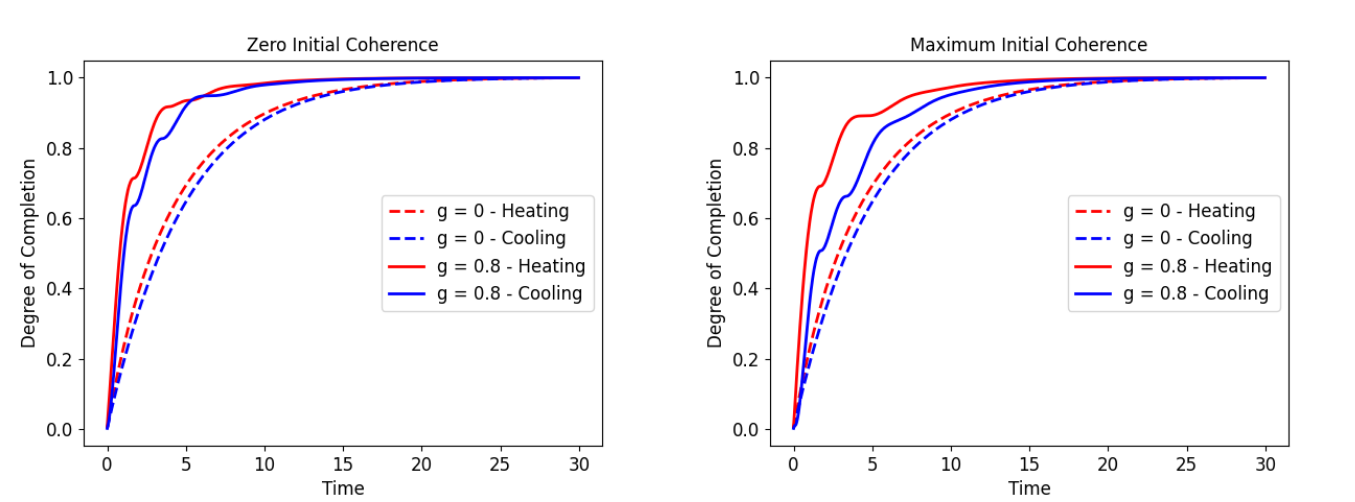
\includegraphics[width=0.8\linewidth]{Images/Qubits/XX/completion-xx.png}
    \caption{Degree of completion for XX-model. Each line correspond to cooling (blue) or heating (red) processes with (solid) or without (dashed) interaction between qubits.}
    \label{fig:completion-xx}
\end{figure}

\begin{figure}[t]
    \centering
    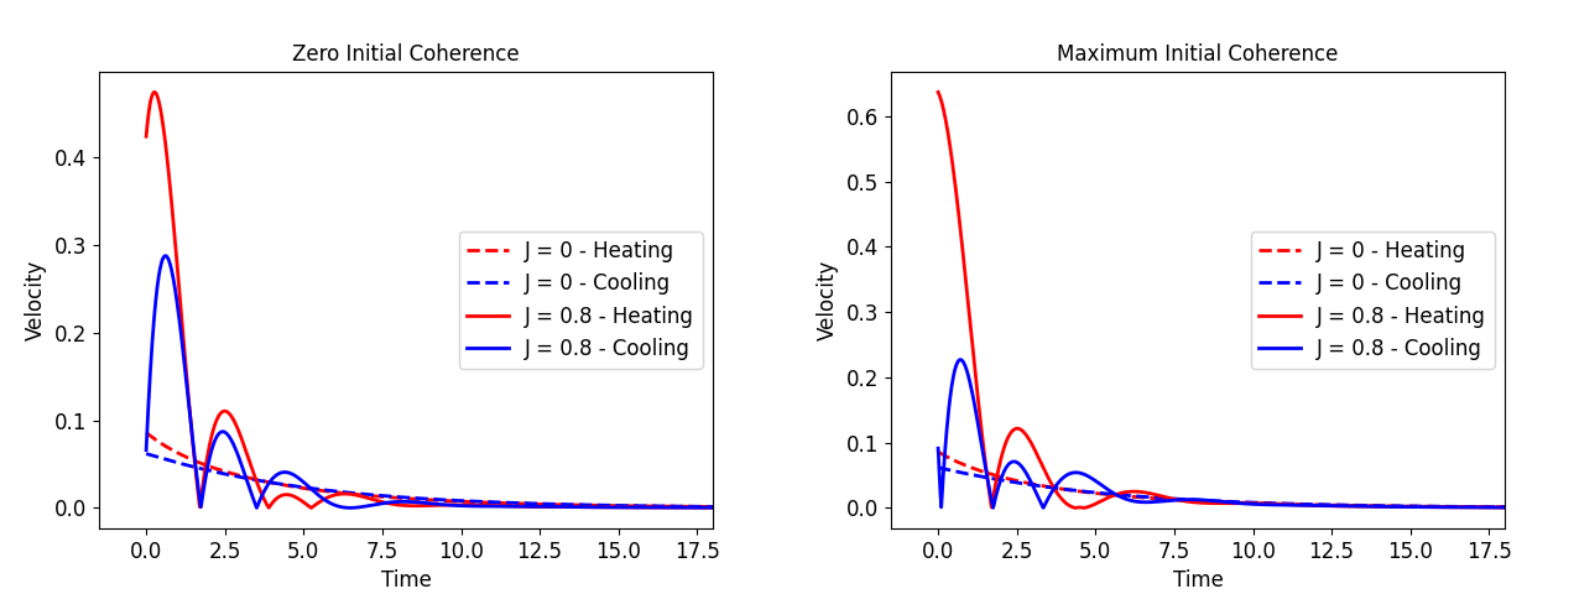
\includegraphics[width=0.8\linewidth]{Images/Qubits/XX/velocity-xx.png}
    \caption{Statistical velocity for XX-model. Each line correspond to cooling (blue) or heating (red) processes with (solid) or without (dashed) interaction between qubits.}
    \label{fig:velocity-xx}
\end{figure}

Previous works have stated that heating is faster than cooling because it has higher entropy production \cite{tejero-misc-2025, ibanez-2024}. As we noticed that the interaction case relaxate faster than the no-interaction case, we could try to also use the argument that the faster process has higher entropy production. In Fig. \ref{fig:sprod-xx}, we show the entropy production rate (defined in Eq. \eqref{eq:sprod}) as a function of time. First, heating without interaction have higher entropy production than cooling which agrees with previous works \cite{tejero-misc-2025, ibanez-2024}. However, the interaction case have many oscillations and heating entropy production is not always bigger than cooling entropy production. Additionally, the entropy production of the interaction case becomes negative for some time intervals. If we recall that entropy is related to the lack of information, negative entropy production means the system is gaining information instead of losing to the environment, which seems like a violation of the second law of thermodynamics. This gain of information is also called information backflow and is related with non-Markovian dynamics \cite{breuer-2015}. However, we are using a global Markovian master equation as defined in Chap. \ref{cap:oqs}. A possible explanation to this dichotomy is that, by limiting our observation to a subpart of the system, we also ignore correlations with the other part, which can seem like memory effects \cite{popovic-2018}. This problem have already been studied before and it was shown that negative entropy production can be a witness of non-Markovianity \cite{popovic-2018, marcantoni-2017}. So a conclusion from this analysis is that non-Markovianity may help the systems to have faster relaxation.

\begin{figure}[t]
    \centering
    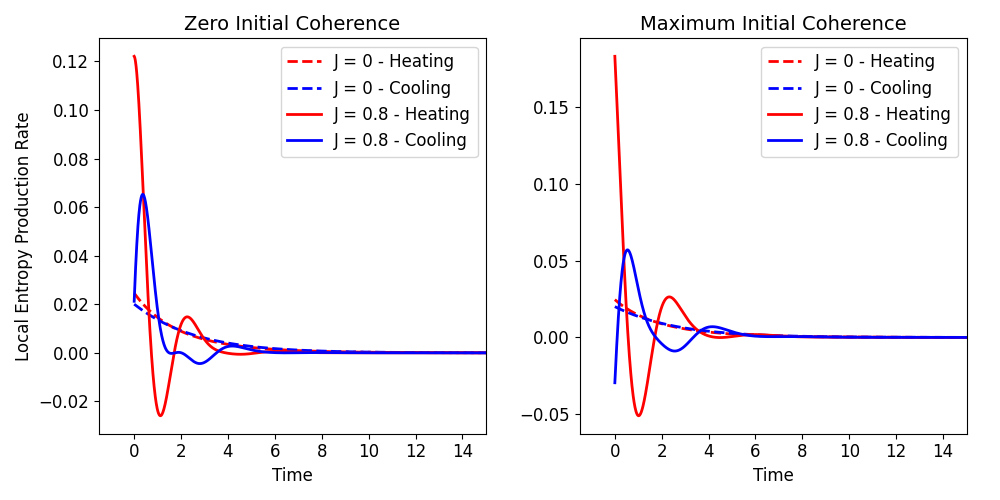
\includegraphics[width=0.8\linewidth]{Images/Qubits/XX/sprod-xx.png}
    \caption{Entropy production rate for the XX-model. Each line corresponds to cooling (blue) or heating (red) processes with (solid) or without (dashed) interaction between qubits.}
    \label{fig:sprod-xx}
\end{figure}

Until this point, we have only discussed an interaction case that do not generate entanglement between the qubits. According to Fig. \ref{fig:C-EoF-MI}, we can increase $J$ to obtain a final entangled state for the qubits. Choosing $J=1.6$, Fig. \ref{fig:completion-all-J-xx} show that the presence of entanglement (dotted lines) reduces the heating-cooling asymmetry making the curves closer. Again the initial coherence do not change the overall thermalisation for $J=1.6$. When compared to our previous interaction case without entanglement (solid lines), we notice that the thermal relaxation becomes slower, but it is still faster than the non-interacting case (dashed lines). Therefore, the relation between the acceleration of thermal relaxation and the increase of $J$ it is not straightforward.

\begin{figure}[t]
    \centering
    
\includegraphics[width=0.9\linewidth]{Images/Qubits/XX/completion-assimetria-xx.png}
    \caption{Degree of completion for heating (red) and cooling (blue) states with zero (left) or maximum (right) initial coherence. The interaction parameters used are $J=0$ (dashed), $J=0.8$ (solid), and $J=1.6$ (dotted).}
    \label{fig:completion-all-J-xx}
\end{figure}
